%você pode organizar melhor suas imagens se criar subpastas nos chapters
\begin{figure}[ht!]
\centering

\caption{\textmd{Fluxograma que ilustra o processo de seleção dos artigos.}}

\label{fig:fluxograma_metodologia}
\fcolorbox{gray}{white}{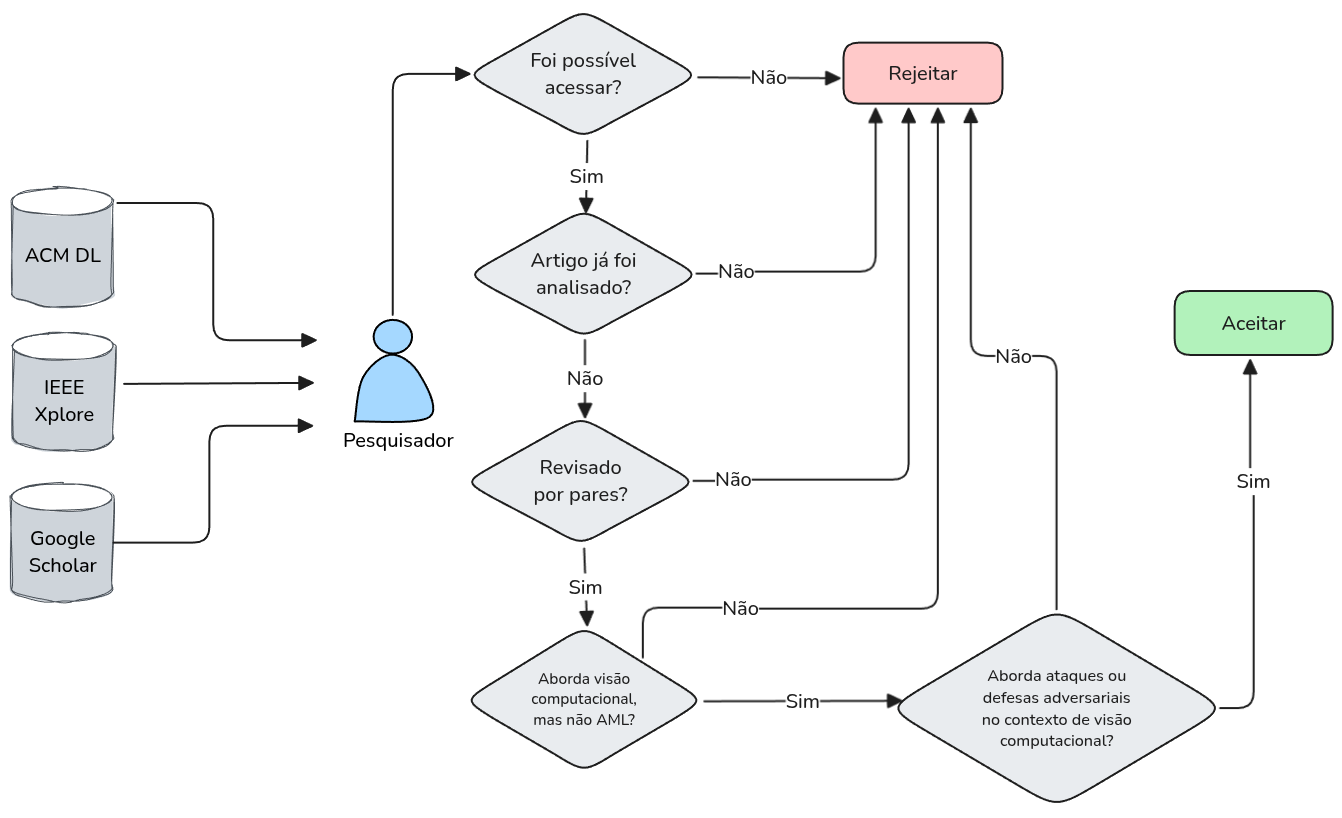
\includegraphics[width=0.9\textwidth]{images/metodologia/fluxograma.png}}

\fonteref{Elaborado pelo autor.}
\end{figure}